%; whizzy paragraph -pdf xpdf -latex ./whizzypdfptex.sh
%; whizzy-paragraph "^\\\\begin{frame}\\|\\\\emtext"
% latex beamer presentation.
% platex, latex-beamer でコンパイルすることを想定。 

%     Tokyo Debian Meeting resources
%     Copyright (C) 2012 Junichi Uekawa
%     Copyright (C) 2014, 2015 Nobuhiro Iwamatsu

%     This program is free software; you can redistribute it and/or modify
%     it under the terms of the GNU General Public License as published by
%     the Free Software Foundation; either version 2 of the License, or
%     (at your option) any later version.

%     This program is distributed in the hope that it will be useful,
%     but WITHOUT ANY WARRANTY; without even the implied warreanty of
%     MERCHANTABILITY or FITNESS FOR A PARTICULAR PURPOSE.  See the
%     GNU General Public License for more details.

%     You should have received a copy of the GNU General Public License
%     along with this program; if not, write to the Free Software
%     Foundation, Inc., 51 Franklin St, Fifth Floor, Boston, MA  02110-1301 USA

\documentclass[cjk,dvipdfmx,12pt]{beamer}
\usetheme{Tokyo}
\usepackage{monthlypresentation}

%  preview (shell-command (concat "evince " (replace-regexp-in-string "tex$" "pdf"(buffer-file-name)) "&")) 
%  presentation (shell-command (concat "xpdf -fullscreen " (replace-regexp-in-string "tex$" "pdf"(buffer-file-name)) "&"))
%  presentation (shell-command (concat "evince " (replace-regexp-in-string "tex$" "pdf"(buffer-file-name)) "&"))

%http://www.naney.org/diki/dk/hyperref.html
%日本語EUC系環境の時
\AtBeginDvi{\special{pdf:tounicode EUC-UCS2}}
%シフトJIS系環境の時
%\AtBeginDvi{\special{pdf:tounicode 90ms-RKSJ-UCS2}}

\newenvironment{commandlinesmall}%
{\VerbatimEnvironment
  \begin{Sbox}\begin{minipage}{1.0\hsize}\begin{fontsize}{8}{8} \begin{BVerbatim}}%
{\end{BVerbatim}\end{fontsize}\end{minipage}\end{Sbox}
  \setlength{\fboxsep}{8pt}
% start on a new paragraph

\vspace{6pt}% skip before
\fcolorbox{dancerdarkblue}{dancerlightblue}{\TheSbox}

\vspace{6pt}% skip after
}
%end of commandlinesmall

\if 0
書くこと

Updates
Newcomer tag in BTS

\fi

\title{東京エリアDebian勉強会}
\subtitle{第124回 2015年2月度\\OSC 2015 Tokyo/Spring 出張勉強会}
\author{岩松 信洋 / iwamatsu@debian.org}
\date{2015年2月28日}
\logo{
\includegraphics[width=8cm]{image200607/openlogo-light.eps}}

\begin{document}

\begin{frame}
\titlepage{}
\end{frame}

\begin{frame}{Agenda}
  \begin{itemize}
   \item Debian Update
   \item Debian 8 状況
   \item 質疑応答
   \item おしらせ
  \end{itemize}
\end{frame}

%
%\begin{block}{ブロック}
%\end{block}
%\begin{alertblock}{警告ブロック}
%\end{alertblock}
%\begin{exampleblock}{例ブロック}
%\end{exampleblock}
%

\begin{frame}{Who am I?}

\begin{itemize}
\item Debian Project 公式開発者
\begin{itemize}
\item linux kernel、ARM、SH4、Mactel チーム
\item Bluez, NFC, Mozc, OpenCV, Erlang
\end{itemize}
\item 普段は Linux カーネル、ブートローダ、BSP(Yocto, OE)の開発
\item U-Boot SH, rmobile メンテナ
\item Yocto Project meta-renesas メンテナ
\end{itemize}

\end{frame}

\emtext{Debian Updates}

\begin{frame}{ポイントリリース}

\begin{itemize}
\item Debian 7 更新状況 (Wheezy)
\begin{itemize}
\item 2014年10月18日 Debian 7 更新: 7.7 リリース\\
      45個のパッケージ修正、73個のセキュリティバグの修正
\item 2015年1月12日 Debian 7 更新: 7.8 リリース\\
      32個のパッケージ修正、87個のセキュリティバグの修正
\end{itemize}
\item Debian 6 更新状況 (Squeeze)
\begin{itemize}
\item なし
\end{itemize}
\end{itemize}

\begin{center}
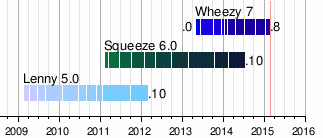
\includegraphics[scale=0.7]{image201502/debian-release-201502-cut.jpg}
\end{center}

\end{frame}

\begin{frame}{アジア初Debian セキュリティミラーサーバ}
\begin{itemize}
\item さくらインターネットさんの協力の元、アジアに初めてのDebianセキュリティミラーサーバが立ち上がる
\item これによってセキュリティ修正を含んだパッケージの頒布/更新遅延が改善されます
\item Debian Developer のやまねさん(@henrich)が交渉交渉してくれました
\item さくらインターネットさん、ありがとうございます!
\end{itemize}
\end{frame}


\begin{frame}{再ビルドチェックチーム}
\begin{itemize}
\item \url{https://wiki.debian.org/ReproducibleBuilds}
\item 長い間ビルドされていないパッケージを最新の環境で再ビルドチェックするチーム
\item アーキテクチャ依存パッケージだけではなく、アーキテクチャに依存しないのパッケージ
(データやフォントなど)も対象
\item 現時点で約83\% のパッケージが再ビルド可能
\item 次のステップとして、ビルド時の情報(ビルド依存パッケージ情報など)を deb
パッケージに含めて情報管理する仕組みを検討
\url(https://wiki.debian.org/ReproducibleBuilds/BuildinfoSpecification)
\end{itemize}
\end{frame}

\begin{frame}{Devuan プロジェクト}

\begin{center}

\includegraphics[scale=0.2]{image201502/devuan.jpg}
\end{center}

\begin{itemize}
\item Debian の init system 対応に疑問を感じた人たちが Debianをフォークし、Devuan
プロジェクトなるものを立ち上げ(\url{https://devuan.org/})
\item ConsoleKit2、policykit-1 などのソフトウェアからsystemd依存部を排除し、パッケージ化するなどの活動をしている
\item とりあえず活動しているが、今後どのような動きをするかは不明。
\end{itemize}

\end{frame}

\begin{frame}{General Resolution: init system coupling}

\begin{itemize}
\item sytemd 以外 の init system のサポートをパッケージメンテナに求める一般決議
\begin{enumerate}
\item パッケージは基本的には特定の init system に依存しない
\item 強制ではないが複数のinit system をサポートする事が推奨される
\item パッケージメンテナは特定のinit sytem への依存を選択できる
\item 一般決議は必要ない
\end{enumerate}
\item 結果は「4. 一般決議は必要ない」となった 

\end{itemize}

\end{frame}

\begin{frame}{2048 bit 以上のGPGキーの更新}
\begin{itemize}
\item より強いGPGキーでWeb of Trust を構築するために、2048bit
以上のキーに更新を要請。
\item 1024bit / DSA などのキーを使っているDebian Developer / Debian Maintaier
は活動できなくなった。(もちろんキーメンテナのよる対応あり)
\end{itemize}

%\begin{center}
%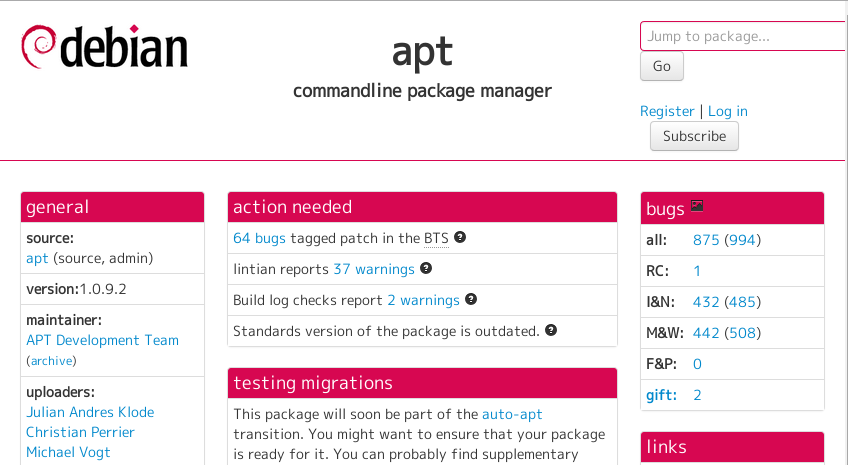
\includegraphics[scale=0.3]{image201410/tracker.png}
%\end{center}

\end{frame}

\emtext{Debian 8.0 状況}

\begin{frame}{フリーズ}
\begin{center}
絶賛フリーズ中
\end{center}
\end{frame}
 
\begin{frame}{フリーズ}
\begin{minipage}{0.55\hsize}
\begin{itemize}
\item 11/5 にフリーズ!
\item フリーズ: パッケージの新しいバージョンへの更新を停止
\begin{itemize}
\item 9/5 にABI更新をフリーズ
\item 10/5 から testing へのマイグレーションを5日から10日に切り替え
\item 着々とバグ潰しが進行中
\end{itemize}
\end{itemize}
\end{minipage}
\begin{minipage}{0.39\hsize}
\begin{center}
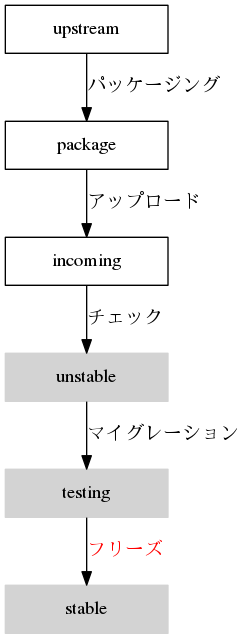
\includegraphics[scale=0.3]{image201410/lifesycle-package.png}
\end{center}
\end{minipage}
\end{frame}

\begin{frame}{バグの数}
\begin{center}
あと 35 個!
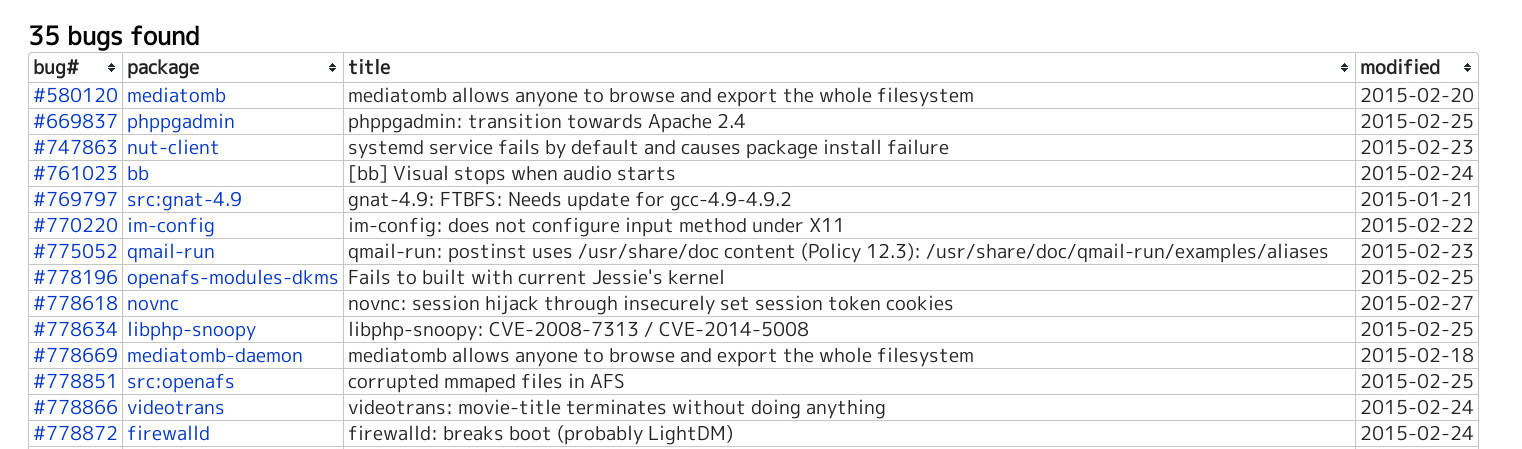
\includegraphics[scale=0.3]{image201502/20150228-rcbugs-cut.jpg}
\end{center}
\end{frame}

\begin{frame}{リリースゴール}
\begin{itemize}
\item systemd
\item piuparts
\item SELinux
\item CrossToolchains
\item CrossBuildableBase
\item utf-8
\item debian/rules honor CC and CXX
\item Clang as secondary compiler
\item Security hardening build flags
\end{itemize}
\end{frame}


\begin{frame}{リリースゴールからはずされたもの}
\begin{itemize}
\item pkg-php-tools 移行(PEAR:PHP Extension and Application Repositoryサポート)
\end{itemize}
\end{frame}

\begin{frame}{サポートアーキテクチャ}

\begin{itemize}
\item IN:
  \begin{itemize}
  \item arm64, ppcel64 がリリースアーキテクチャ入り。
  %\item \url{https://lists.debian.org/debian-devel-announce/2014/09/msg00002.html}
  \item x32 は入らなかった。
  \end{itemize}
\item OUT: ia64、sparc、s390
\begin{itemize}
\item ia64 はdebian-ports でメンテナンス
\item s390 は s390x に移行
\end{itemize}
\end{itemize}

\end{frame}

\begin{frame}{デフォルト init システム}

\begin{itemize}
\item Linux のデフォルトの init システムが systemd に
\item minimal でインストールしても /sbin/init が systemd
\end{itemize}

\end{frame}

\begin{frame}{主要ソフトウェアの更新状況}

\begin{itemize}
\item Linux kernel: 3.16.x (4.0-rc1)
\item kFreeBSD: 8,9,10 (11)
\end{itemize}

\end{frame}

\begin{frame}{主要ソフトウェアの更新状況}
\begin{itemize}
\item GNOME: 3.14 (3.14)
\item KDE: 4.14.2 (4.14.3)
\item Xfce: 4.10 (4.10)
\item LXDE: 0.7.2 (lxqt 0.9.0)
\item MATE: 1.8.0 (1.8.0)
\item Cinnamon: 2.2.16 (2.2.16)
\end{itemize}
\end{frame}

\begin{frame}{主要ソフトウェアの更新状況}
\begin{itemize}
\item Toolchain: GCC:4.9.1. binutils: 2.24.51, glibc: 2:19
\item LLVM: 3.4.2, 3.5.0 (3.6.0)
\item Perl: 5.20.1 (5.20.2)
\item Ruby: 2.1.5 (2.2.0.rc1)
\item Python2: 2.7.9 (2.7.9)
\item Python3: 3.4.2 (3.4.3)
\item PHP: 5.6.5 (5.6.6)
\item Lua: 5.2.3 (5.3.0)
\item ghc: 7.6.3 (7.10.0)
\end{itemize}
\end{frame}

\begin{frame}{主要ソフトウェアの更新状況}
\begin{itemize}
\item Xorg: 1.16.4 (1.17.1)
\item Wayland: 1.6.0 (1.7.0)
\item systemd: 215 (219)
\item Emacs: 24.4 (24.4)
\item Vim: 7.4.488 (7.4.646)
\item Pulseaudio: 5.0 (6.0)
\item Apache: 2.4.10 (2.4.12)
\item VLC: 2.2.0$~$rc2 (2.2.0) 
\item zabbix: 2.2.7 (2.4.3)
\end{itemize}

\end{frame}

\begin{frame}{主要ソフトウェアの更新状況}
\begin{itemize}
\item rails: 4.1.8 (4.2.0)
\item django: 1.7.4 (1.7.5)
\item QEMU: 2.1 (2.2)
\item lxc: 1.0.6 (1.1.0)
\item mysql 5.5.42 (5.6.23)
\item mariadb 10.0.16 (10.0.16)
\item postgresql 9.4.1 (9.4.1)
\end{itemize}

\end{frame}
\begin{frame}[containsverbatim]{Debian Installer Jessie RC 1 release}
\begin{itemize}
\item 2015年1月26日 に Debian Installer Jessie RC 1がリリース
\item QEMU などで気軽に試せます
\item OSC Debian ブースでも頒布しています
\end{itemize}
\end{frame}

\begin{frame}{まとめ}
\begin{itemize}
\item 11/5
にフリーズし、絶賛デバッグ中。リリースためにはバグを35個潰す必要がある
\item arm64, ppcel64がリリースアーキテクチャ入り
\item 主要パッケージは比較的新しいものが入る
\item Debian 8 用インストーラがRC1としてリリース。テストできる環境は
整っている
\end{itemize}
\end{frame}

\begin{frame}{リリースに向けてお願い}
\begin{itemize}
\item テストにご協力ください。インストールレポート、ソフトウェア動作レポート、
未翻訳など報告していただけると非常に助かります。
\end{itemize}

\end{frame}

\emtext{Debian 8 の次は?}

\begin{frame}{Debian 8 の次は?}
\begin{itemize}
\item Debian 9 のコードネームは Stretch
\end{itemize}

%\begin{center}
%  \includegraphics[scale=0.8]{image201502/stretch.jpg}
%\end{center}

\end{frame}

\begin{frame}{Debian 8 の次は?}
  \begin{itemize}
  \item Debian 10 のコードネームは Buster
  \end{itemize}

%  \begin{center}
%    \includegraphics[scale=0.8]{image201502/buster.jpg}
%  \end{center}

\end{frame}

\begin{frame}[containsverbatim]{質問}

\begin{center}
なにか質問はありますか?
\end{center}

\end{frame}

\begin{frame}{おしらせ}
\begin{itemize}
\item ブース出展中
\begin{itemize}
\item Debian 起動 マシン展示(NUC, 96boards Hikey, Raspberry Pi 2)
\item ステッカー、チラシ、インストーラCD配布
\item Debianに関する相談受付
\item GPGサイン、CAcertサイン
\end{itemize}
\end{itemize}

\end{frame}

\begin{frame}{次回の勉強会}
\begin{itemize}
\item 次回勉強会は 3/7(土)14:00-19:00 スクエアエニックスさん セミナールーム
\item 内容は未定
\item 聞きたい話があったら相談ください
\item その他情報は Debian JP Project サイト \url{http://www.debian.or.jp}または Twitter:@debianjp にて
\end{itemize}
\end{frame}


\begin{frame}{利用画像等}
\begin{itemize}
\item
\url{http://upload.wikimedia.org/wikipedia/en/timeline/ed3c27abacc3656e55150a75faed2221.png}
\end{itemize}
\end{frame}

\end{document}

;;; Local Variables: ***
;;; outline-regexp: "\\([ 	]*\\\\\\(documentstyle\\|documentclass\\|emtext\\|section\\|begin{frame}\\)\\*?[ 	]*[[{]\\|[]+\\)" ***
;;; End: ***



%------

